%==============================================================
%  Figura 6.15 - Schema di principio dell'azionamento elettronico di
%  una lama idraulica e di una barra di pressione idraulica
%  Adattamento in italiano della Figura 6.15 dell'IFA Report 2/2017
%
%  Nell'originale questa figura e' un'immagine raster incorporata che
%  contiene SOLO il disegno: tutte le scritte (diciture e sigle dei
%  componenti) stanno in un livello di testo separato. Qui si fa
%  altrettanto: img06-15.png e' il disegno estratto dall'originale
%  (pagina 76 di rep0217e.pdf, 1877x2776 px a 300 ppi) e le scritte
%  sono nodi TikZ sovrapposti, quindi restano testo selezionabile e
%  sono state tradotte senza ritoccare il bitmap.
%
%  Le posizioni dei nodi sono quelle misurate nell'originale.
%  Sistema di riferimento: l'origine e' l'angolo in basso a sinistra
%  della cornice, l'asse y e' rivolto verso l'alto e una unita' e' un
%  punto PostScript del disegno originale.
%==============================================================
\begin{tikzpicture}[
  x=0.035cm, y=0.035cm,
  grande/.style={font=\fontsize{10.2}{12}\selectfont},
  media/.style={font=\fontsize{8.5}{10}\selectfont},
  piccola/.style={font=\fontsize{7.6}{9}\selectfont}
]

\setstretch{1}

% --- disegno (bitmap estratto dall'originale, privo di scritte) ---
\node[anchor=south west, inner sep=0] at (22.69,6.39)
  {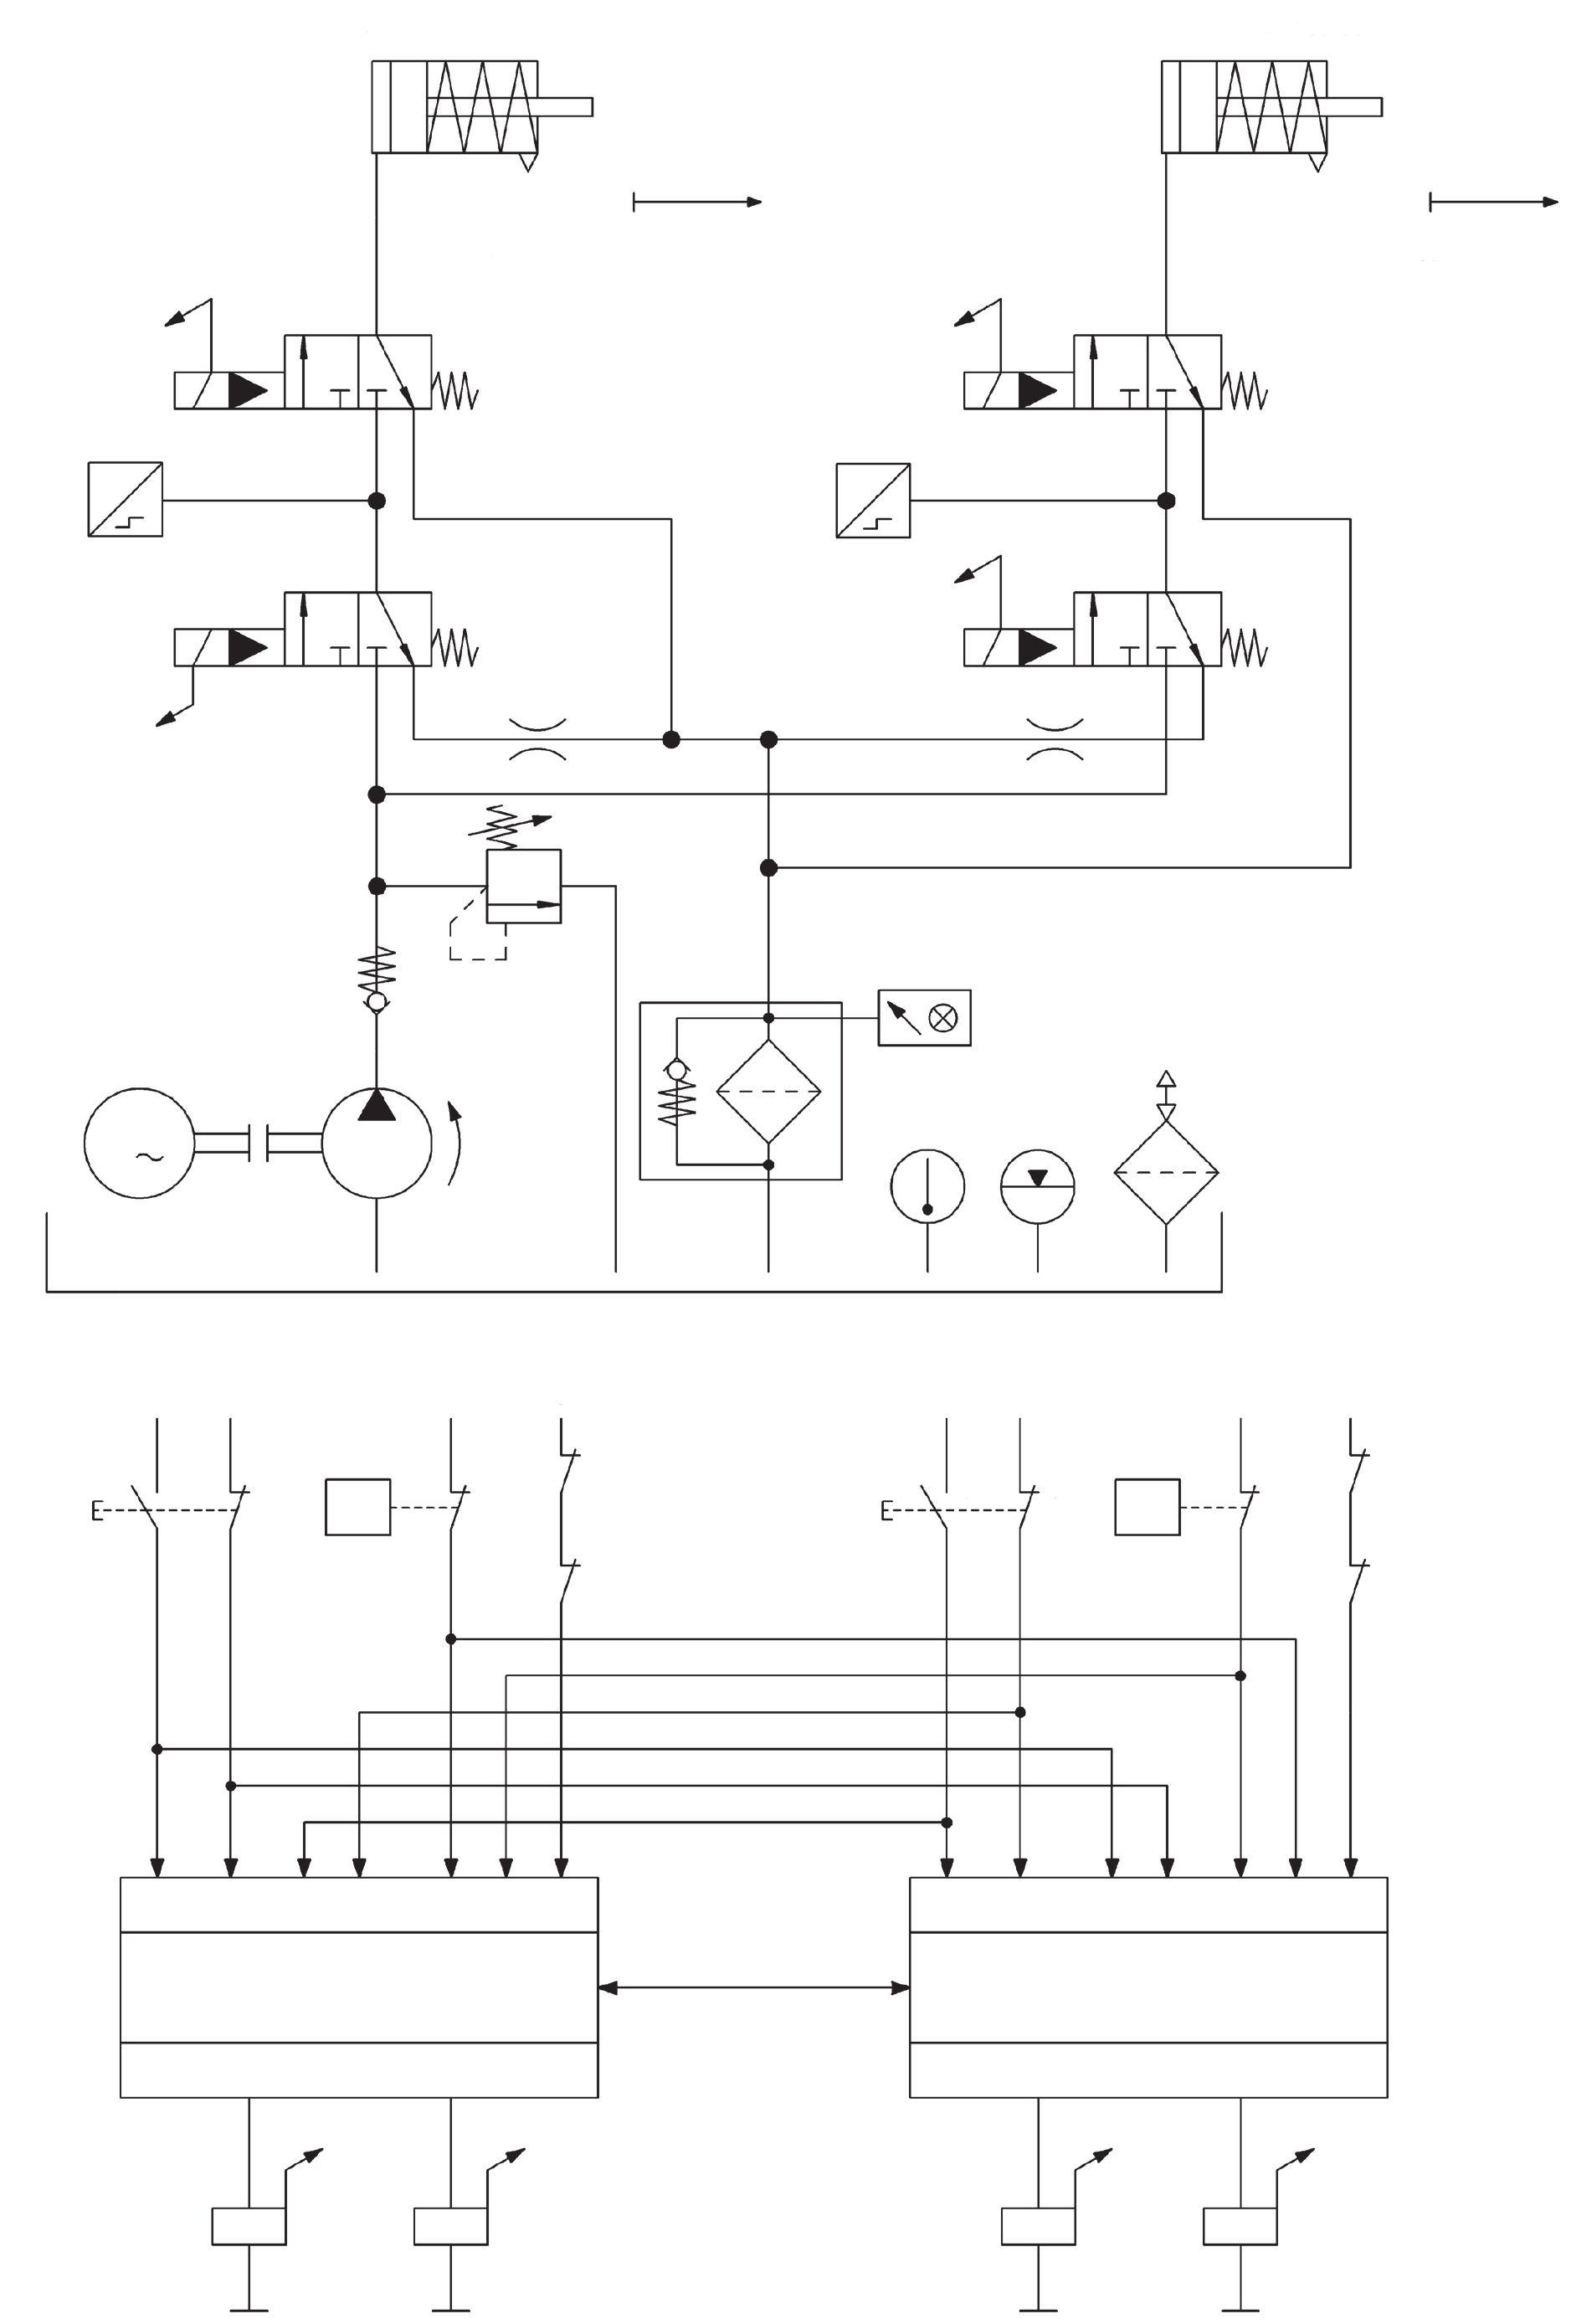
\includegraphics[width=15.740cm, height=23.289cm]{img06-15.png}};

% --- scritte: diciture tradotte e sigle dei componenti ---
\node[grande] at (153.06,661.35) {Azionamento della lama};
\node[grande] at (385.72,661.35) {Barra di pressione};
\node[media] at (121.89,641.37) {1A};
\node[media] at (348.32,641.37) {2A};
\node[grande, align=center] at (225.54,596.72) {Movimento\\pericoloso};
\node[grande, align=center] at (446.75,596.72) {Movimento\\pericoloso};
\node[media] at (290.19,578.77) {K4};
\node[media] at (64.14,577.83) {K3};
\node[media] at (62.25,561.48) {1V4};
\node[media] at (288.83,560.08) {2V2};
\node[media] at (54.92,533.22) {P};
\node[media] at (270.05,533.22) {P};
\node[media] at (39.65,530.42) {1S3};
\node[media] at (251.99,528.78) {2S1};
\node[media] at (290.24,504.02) {K6};
\node[media] at (63.93,486.97) {1V3};
\node[media] at (288.66,486.97) {2V1};
\node[media] at (177.03,471.55) {1V5};
\node[media] at (326.88,471.55) {2V3};
\node[media] at (61.86,463.85) {K5};
\node[media] at (152.71,424.61) {1V2};
\node[media] at (117.51,391.91) {1V1};
\node[media] at (213.40,389.80) {1Z2};
\node[media] at (347.14,364.27) {1Z1};
\node[media] at (62.67,350.80) {M};
\node[media] at (288.65,347.29) {1S1};
\node[media] at (319.81,347.29) {1S2};
\node[media] at (39.70,344.56) {1M};
\node[media] at (164.79,344.56) {1P};
\node[media] at (58.55,340.52) {3};
\node[media] at (68.19,273.17) {+};
\node[media] at (88.51,273.17) {+};
\node[media] at (151.73,273.17) {+};
\node[media] at (183.81,273.17) {+};
\node[media] at (294.06,273.17) {+};
\node[media] at (315.39,273.17) {+};
\node[media] at (378.29,273.17) {+};
\node[media] at (409.43,273.17) {+};
\node[media] at (125.76,254.49) {1S3};
\node[media] at (351.97,254.48) {2S1};
\node[media] at (175.14,250.75) {K5};
\node[media] at (402.66,249.50) {K3};
\node[piccola] at (76.90,245.46) {13};
\node[piccola] at (305.03,245.15) {13};
\node[piccola] at (100.28,244.84) {21};
\node[piccola] at (328.41,244.53) {21};
\node[grande] at (125.81,240.14) {P\textgreater{}};
\node[grande] at (351.92,240.14) {P\textgreater{}};
\node[media] at (40.98,239.54) {S1};
\node[media] at (268.03,239.54) {S2};
\node[piccola] at (77.07,233.63) {14};
\node[piccola] at (100.86,233.63) {22};
\node[piccola] at (305.19,233.32) {14};
\node[piccola] at (328.98,233.32) {22};
\node[media] at (175.54,219.61) {K6};
\node[media] at (402.86,218.35) {K4};
\node[media] at (45.39,127.10) {K1};
\node[media] at (272.53,127.10) {K2};
\node[media] at (348.66,125.24) {Ingresso};
\node[media] at (116.32,125.24) {Ingresso};
\node[grande] at (352.38,104.97) {ASIC};
\node[grande] at (121.69,103.73) {Microcontrollore};
\node[media, align=center] at (239.52,102.35) {Sincronizzazione e\\scambio di dati};
\node[media] at (119.66,78.83) {Uscita};
\node[media] at (351.99,78.83) {Uscita};
\node[media] at (115.49,61.40) {1V4};
\node[media] at (174.54,61.39) {2V2};
\node[media] at (342.68,61.39) {1V3};
\node[media] at (399.69,61.39) {2V1};
\node[media] at (134.62,34.61) {K4};
\node[media] at (74.35,34.60) {K3};
\node[media] at (302.22,34.60) {K5};
\node[media] at (360.56,34.60) {K6};

% --- cornice esterna ---
\draw[draw=black, line width=0.75pt] (0.37,0.37) rectangle (497.93,677.81);

\end{tikzpicture}
